% Real archived PushT example; source macros and PNGs preserved.
% Generated by scripts/cta_fig1_tex.py from /mnt/data/nhatnc129/jepa/trajectory_innovation/cta_fig1_55314/r2102_d16 (root 2102, decision 16, t = 128). Do not edit by hand.
% CTA choice 7, best label 7, worst label 4 (1-based); labels (mean vertex error, px) 16.6, 18.4, 24.0, 28.0, 27.3, 22.1, 15.2, 18.7
\def\FigChosen{7}\def\FigBest{7}\def\FigWorst{4}
\def\FigChosenIdx{6}\def\FigBestIdx{6}\def\FigWorstIdx{3}
\def\FigGoals{0,1,2}
\def\FigErrBest{15}\def\FigErrWorst{28}
\newcommand{\FigImgTop}[2]{\includegraphics[width=#1,trim=97.1 95.1 199.6 201.6,clip]{fig/pusht/#2}}
\newcommand{\FigImgProp}[2]{\includegraphics[width=#1,trim=75.6 72.1 316.4 319.9,clip]{fig/pusht/#2}}
\newcommand{\FigImgBottom}[2]{\includegraphics[width=#1,trim=108.6 106.2 201.3 203.6,clip]{fig/pusht/#2}}
\def\FigZoomTop{(0.1897,0.1858) rectangle (0.6102,0.6063)}
\def\FigZoomProp{(0.1477,0.1408) rectangle (0.3821,0.3752)}
\newcommand{\FigPathsTop}{%
  \draw[proposal] (0.0901,0.0557) -- (0.1642,0.1156) -- (0.1849,0.1426) -- (0.2056,0.1659) -- (0.2204,0.1825) -- (0.2331,0.2056) -- (0.2450,0.2284) -- (0.2577,0.2515) -- (0.2676,0.2735);
  \draw[proposal] (0.0901,0.0557) -- (0.1544,0.1177) -- (0.1731,0.1475) -- (0.1893,0.1719) -- (0.2001,0.1911) -- (0.2119,0.2129) -- (0.2249,0.2303) -- (0.2407,0.2522) -- (0.2556,0.2790);
  \draw[proposal] (0.0901,0.0557) -- (0.1535,0.1189) -- (0.1701,0.1426) -- (0.1824,0.1626) -- (0.1917,0.1786) -- (0.1982,0.1979) -- (0.2083,0.2135) -- (0.2216,0.2306) -- (0.2366,0.2529);
  \draw[proposal] (0.0901,0.0557) -- (0.1396,0.1101) -- (0.1526,0.1281) -- (0.1601,0.1453) -- (0.1637,0.1582) -- (0.1692,0.1847) -- (0.1787,0.2159) -- (0.1935,0.2397) -- (0.2072,0.2581);
  \draw[proposal] (0.0901,0.0557) -- (0.1379,0.1060) -- (0.1523,0.1240) -- (0.1675,0.1463) -- (0.1773,0.1636) -- (0.1837,0.1793) -- (0.1960,0.1992) -- (0.2082,0.2262) -- (0.2188,0.2524);
  \draw[proposal] (0.0901,0.0557) -- (0.1485,0.1169) -- (0.1612,0.1386) -- (0.1661,0.1576) -- (0.1711,0.1779) -- (0.1817,0.2079) -- (0.1970,0.2359) -- (0.2176,0.2574) -- (0.2321,0.2747);
  \draw[proposal] (0.0901,0.0557) -- (0.1483,0.1137) -- (0.1661,0.1396) -- (0.1812,0.1624) -- (0.1912,0.1824) -- (0.2027,0.2088) -- (0.2136,0.2363) -- (0.2307,0.2643) -- (0.2480,0.2879);
  \draw[chosenhalo] (0.0901,0.0557) -- (0.1616,0.1172) -- (0.1806,0.1463) -- (0.1995,0.1688) -- (0.2181,0.1889) -- (0.2332,0.2147) -- (0.2428,0.2399) -- (0.2532,0.2639) -- (0.2658,0.2852);
  \draw[chosen] (0.0901,0.0557) -- (0.1616,0.1172) -- (0.1806,0.1463) -- (0.1995,0.1688) -- (0.2181,0.1889) -- (0.2332,0.2147) -- (0.2428,0.2399) -- (0.2532,0.2639) -- (0.2658,0.2852);}
\newcommand{\FigPathsProp}{%
  \draw[proposal] (0.3407,0.2917) -- (0.4737,0.3992) -- (0.5109,0.4475) -- (0.5480,0.4894) -- (0.5745,0.5191) -- (0.5974,0.5606) -- (0.6188,0.6015) -- (0.6416,0.6430) -- (0.6593,0.6825);
  \draw[proposal] (0.3407,0.2917) -- (0.4562,0.4029) -- (0.4897,0.4563) -- (0.5187,0.5002) -- (0.5382,0.5345) -- (0.5593,0.5738) -- (0.5827,0.6050) -- (0.6111,0.6442) -- (0.6377,0.6922);
  \draw[proposal] (0.3407,0.2917) -- (0.4545,0.4051) -- (0.4843,0.4475) -- (0.5064,0.4834) -- (0.5232,0.5121) -- (0.5347,0.5467) -- (0.5529,0.5748) -- (0.5768,0.6054) -- (0.6036,0.6454);
  \draw[proposal] (0.3407,0.2917) -- (0.4295,0.3893) -- (0.4530,0.4215) -- (0.4663,0.4523) -- (0.4728,0.4756) -- (0.4828,0.5230) -- (0.4997,0.5792) -- (0.5263,0.6217) -- (0.5509,0.6548);
  \draw[proposal] (0.3407,0.2917) -- (0.4266,0.3819) -- (0.4525,0.4141) -- (0.4796,0.4541) -- (0.4972,0.4852) -- (0.5087,0.5133) -- (0.5309,0.5490) -- (0.5527,0.5975) -- (0.5717,0.6446);
  \draw[proposal] (0.3407,0.2917) -- (0.4456,0.4014) -- (0.4684,0.4403) -- (0.4772,0.4745) -- (0.4862,0.5109) -- (0.5051,0.5646) -- (0.5325,0.6150) -- (0.5695,0.6535) -- (0.5956,0.6846);
  \draw[proposal] (0.3407,0.2917) -- (0.4453,0.3957) -- (0.4771,0.4421) -- (0.5043,0.4830) -- (0.5222,0.5190) -- (0.5428,0.5664) -- (0.5624,0.6157) -- (0.5931,0.6660) -- (0.6241,0.7083);
  \draw[chosenhalo] (0.3407,0.2917) -- (0.4691,0.4020) -- (0.5033,0.4542) -- (0.5372,0.4946) -- (0.5704,0.5306) -- (0.5976,0.5768) -- (0.6147,0.6222) -- (0.6334,0.6653) -- (0.6561,0.7033);
  \draw[chosen] (0.3407,0.2917) -- (0.4691,0.4020) -- (0.5033,0.4542) -- (0.5372,0.4946) -- (0.5704,0.5306) -- (0.5976,0.5768) -- (0.6147,0.6222) -- (0.6334,0.6653) -- (0.6561,0.7033);}
\newcommand{\FigChosenTop}{\draw[chosenhalo] (0.0901,0.0557) -- (0.1616,0.1172) -- (0.1806,0.1463) -- (0.1995,0.1688) -- (0.2181,0.1889) -- (0.2332,0.2147) -- (0.2428,0.2399) -- (0.2532,0.2639) -- (0.2658,0.2852);\draw[chosen] (0.0901,0.0557) -- (0.1616,0.1172) -- (0.1806,0.1463) -- (0.1995,0.1688) -- (0.2181,0.1889) -- (0.2332,0.2147) -- (0.2428,0.2399) -- (0.2532,0.2639) -- (0.2658,0.2852);}
\definecolor{figP0t0}{rgb}{0.678,0.696,0.194}
\definecolor{figP0t1}{rgb}{0.677,0.697,0.191}
\definecolor{figP0t2}{rgb}{0.697,0.690,0.174}
\definecolor{figP0t3}{rgb}{0.677,0.696,0.189}
\definecolor{figP0t4}{rgb}{0.680,0.700,0.191}
\definecolor{figP0t5}{rgb}{0.676,0.699,0.209}
\definecolor{figP0t6}{rgb}{0.684,0.699,0.199}
\definecolor{figP0t7}{rgb}{0.677,0.694,0.189}
\definecolor{figP0t8}{rgb}{0.676,0.691,0.181}
\definecolor{figP0t9}{rgb}{0.678,0.697,0.196}
\definecolor{figP0t10}{rgb}{0.676,0.693,0.179}
\definecolor{figP0t11}{rgb}{0.649,0.693,0.204}
\definecolor{figP0t12}{rgb}{0.694,0.693,0.171}
\definecolor{figP0t13}{rgb}{0.678,0.695,0.191}
\definecolor{figP0t14}{rgb}{0.696,0.691,0.176}
\definecolor{figP0t15}{rgb}{0.680,0.697,0.189}
\definecolor{figP1t0}{rgb}{0.639,0.647,0.178}
\definecolor{figP1t1}{rgb}{0.641,0.648,0.173}
\definecolor{figP1t2}{rgb}{0.662,0.644,0.158}
\definecolor{figP1t3}{rgb}{0.638,0.648,0.172}
\definecolor{figP1t4}{rgb}{0.648,0.658,0.174}
\definecolor{figP1t5}{rgb}{0.637,0.650,0.194}
\definecolor{figP1t6}{rgb}{0.648,0.651,0.182}
\definecolor{figP1t7}{rgb}{0.639,0.644,0.171}
\definecolor{figP1t8}{rgb}{0.641,0.644,0.162}
\definecolor{figP1t9}{rgb}{0.641,0.650,0.180}
\definecolor{figP1t10}{rgb}{0.641,0.645,0.160}
\definecolor{figP1t11}{rgb}{0.612,0.653,0.183}
\definecolor{figP1t12}{rgb}{0.660,0.647,0.155}
\definecolor{figP1t13}{rgb}{0.641,0.648,0.173}
\definecolor{figP1t14}{rgb}{0.663,0.645,0.159}
\definecolor{figP1t15}{rgb}{0.643,0.648,0.171}
\definecolor{figP2t0}{rgb}{0.488,0.513,0.166}
\definecolor{figP2t1}{rgb}{0.489,0.513,0.161}
\definecolor{figP2t2}{rgb}{0.509,0.508,0.152}
\definecolor{figP2t3}{rgb}{0.491,0.514,0.155}
\definecolor{figP2t4}{rgb}{0.501,0.533,0.166}
\definecolor{figP2t5}{rgb}{0.480,0.522,0.182}
\definecolor{figP2t6}{rgb}{0.496,0.519,0.169}
\definecolor{figP2t7}{rgb}{0.487,0.510,0.158}
\definecolor{figP2t8}{rgb}{0.495,0.514,0.155}
\definecolor{figP2t9}{rgb}{0.490,0.516,0.164}
\definecolor{figP2t10}{rgb}{0.496,0.516,0.151}
\definecolor{figP2t11}{rgb}{0.457,0.529,0.162}
\definecolor{figP2t12}{rgb}{0.508,0.512,0.154}
\definecolor{figP2t13}{rgb}{0.493,0.515,0.159}
\definecolor{figP2t14}{rgb}{0.509,0.509,0.154}
\definecolor{figP2t15}{rgb}{0.496,0.517,0.156}
\definecolor{figP3t0}{rgb}{0.388,0.382,0.174}
\definecolor{figP3t1}{rgb}{0.380,0.378,0.169}
\definecolor{figP3t2}{rgb}{0.398,0.370,0.169}
\definecolor{figP3t3}{rgb}{0.386,0.384,0.162}
\definecolor{figP3t4}{rgb}{0.389,0.389,0.175}
\definecolor{figP3t5}{rgb}{0.378,0.385,0.183}
\definecolor{figP3t6}{rgb}{0.390,0.387,0.172}
\definecolor{figP3t7}{rgb}{0.382,0.375,0.166}
\definecolor{figP3t8}{rgb}{0.390,0.385,0.166}
\definecolor{figP3t9}{rgb}{0.386,0.385,0.167}
\definecolor{figP3t10}{rgb}{0.388,0.383,0.163}
\definecolor{figP3t11}{rgb}{0.358,0.380,0.173}
\definecolor{figP3t12}{rgb}{0.401,0.380,0.168}
\definecolor{figP3t13}{rgb}{0.384,0.383,0.165}
\definecolor{figP3t14}{rgb}{0.397,0.370,0.169}
\definecolor{figP3t15}{rgb}{0.388,0.387,0.164}
\definecolor{figP4t0}{rgb}{0.393,0.392,0.183}
\definecolor{figP4t1}{rgb}{0.385,0.389,0.177}
\definecolor{figP4t2}{rgb}{0.406,0.382,0.179}
\definecolor{figP4t3}{rgb}{0.391,0.395,0.171}
\definecolor{figP4t4}{rgb}{0.394,0.399,0.185}
\definecolor{figP4t5}{rgb}{0.384,0.396,0.192}
\definecolor{figP4t6}{rgb}{0.396,0.396,0.181}
\definecolor{figP4t7}{rgb}{0.388,0.386,0.175}
\definecolor{figP4t8}{rgb}{0.396,0.395,0.174}
\definecolor{figP4t9}{rgb}{0.391,0.395,0.175}
\definecolor{figP4t10}{rgb}{0.393,0.393,0.171}
\definecolor{figP4t11}{rgb}{0.361,0.389,0.183}
\definecolor{figP4t12}{rgb}{0.408,0.391,0.178}
\definecolor{figP4t13}{rgb}{0.389,0.393,0.173}
\definecolor{figP4t14}{rgb}{0.407,0.383,0.180}
\definecolor{figP4t15}{rgb}{0.393,0.397,0.171}
\definecolor{figP5t0}{rgb}{0.536,0.550,0.153}
\definecolor{figP5t1}{rgb}{0.539,0.550,0.150}
\definecolor{figP5t2}{rgb}{0.555,0.542,0.136}
\definecolor{figP5t3}{rgb}{0.539,0.549,0.143}
\definecolor{figP5t4}{rgb}{0.548,0.566,0.154}
\definecolor{figP5t5}{rgb}{0.530,0.556,0.170}
\definecolor{figP5t6}{rgb}{0.544,0.554,0.157}
\definecolor{figP5t7}{rgb}{0.536,0.545,0.147}
\definecolor{figP5t8}{rgb}{0.542,0.549,0.142}
\definecolor{figP5t9}{rgb}{0.538,0.551,0.153}
\definecolor{figP5t10}{rgb}{0.543,0.550,0.138}
\definecolor{figP5t11}{rgb}{0.509,0.565,0.149}
\definecolor{figP5t12}{rgb}{0.555,0.548,0.138}
\definecolor{figP5t13}{rgb}{0.542,0.550,0.148}
\definecolor{figP5t14}{rgb}{0.554,0.543,0.137}
\definecolor{figP5t15}{rgb}{0.543,0.551,0.143}
\definecolor{figP6t0}{rgb}{0.703,0.721,0.197}
\definecolor{figP6t1}{rgb}{0.701,0.723,0.194}
\definecolor{figP6t2}{rgb}{0.716,0.715,0.179}
\definecolor{figP6t3}{rgb}{0.700,0.722,0.191}
\definecolor{figP6t4}{rgb}{0.700,0.723,0.194}
\definecolor{figP6t5}{rgb}{0.699,0.725,0.212}
\definecolor{figP6t6}{rgb}{0.706,0.725,0.204}
\definecolor{figP6t7}{rgb}{0.703,0.721,0.191}
\definecolor{figP6t8}{rgb}{0.699,0.717,0.185}
\definecolor{figP6t9}{rgb}{0.700,0.722,0.199}
\definecolor{figP6t10}{rgb}{0.700,0.719,0.184}
\definecolor{figP6t11}{rgb}{0.672,0.715,0.208}
\definecolor{figP6t12}{rgb}{0.713,0.717,0.175}
\definecolor{figP6t13}{rgb}{0.703,0.721,0.194}
\definecolor{figP6t14}{rgb}{0.717,0.717,0.180}
\definecolor{figP6t15}{rgb}{0.703,0.722,0.193}
\definecolor{figP7t0}{rgb}{0.617,0.622,0.169}
\definecolor{figP7t1}{rgb}{0.621,0.623,0.165}
\definecolor{figP7t2}{rgb}{0.639,0.619,0.150}
\definecolor{figP7t3}{rgb}{0.617,0.622,0.162}
\definecolor{figP7t4}{rgb}{0.627,0.633,0.168}
\definecolor{figP7t5}{rgb}{0.614,0.626,0.186}
\definecolor{figP7t6}{rgb}{0.625,0.625,0.175}
\definecolor{figP7t7}{rgb}{0.617,0.619,0.162}
\definecolor{figP7t8}{rgb}{0.620,0.619,0.154}
\definecolor{figP7t9}{rgb}{0.618,0.624,0.172}
\definecolor{figP7t10}{rgb}{0.620,0.621,0.152}
\definecolor{figP7t11}{rgb}{0.590,0.630,0.174}
\definecolor{figP7t12}{rgb}{0.638,0.622,0.149}
\definecolor{figP7t13}{rgb}{0.620,0.623,0.164}
\definecolor{figP7t14}{rgb}{0.640,0.620,0.152}
\definecolor{figP7t15}{rgb}{0.622,0.622,0.161}
\definecolor{figS0t0}{rgb}{0.750,0.750,0.250}
\definecolor{figS0t1}{rgb}{0.750,0.750,0.250}
\definecolor{figS0t2}{rgb}{0.750,0.750,0.000}
\definecolor{figS0t3}{rgb}{0.750,0.750,0.250}
\definecolor{figS0t4}{rgb}{0.750,0.750,0.250}
\definecolor{figS0t5}{rgb}{0.750,0.750,0.250}
\definecolor{figS0t6}{rgb}{0.750,0.750,0.250}
\definecolor{figS0t7}{rgb}{0.750,0.750,0.250}
\definecolor{figS0t8}{rgb}{0.750,0.750,0.250}
\definecolor{figS0t9}{rgb}{0.750,0.750,0.250}
\definecolor{figS0t10}{rgb}{0.750,0.750,0.250}
\definecolor{figS0t11}{rgb}{0.750,0.750,0.250}
\definecolor{figS0t12}{rgb}{0.750,0.750,0.000}
\definecolor{figS0t13}{rgb}{0.750,0.750,0.250}
\definecolor{figS0t14}{rgb}{0.750,0.750,0.000}
\definecolor{figS0t15}{rgb}{0.750,0.750,0.250}
\definecolor{figS1t0}{rgb}{0.500,0.375,0.250}
\definecolor{figS1t1}{rgb}{0.500,0.375,0.250}
\definecolor{figS1t2}{rgb}{0.500,0.375,0.250}
\definecolor{figS1t3}{rgb}{0.500,0.375,0.250}
\definecolor{figS1t4}{rgb}{0.500,0.375,0.250}
\definecolor{figS1t5}{rgb}{0.500,0.375,0.250}
\definecolor{figS1t6}{rgb}{0.500,0.375,0.250}
\definecolor{figS1t7}{rgb}{0.500,0.375,0.250}
\definecolor{figS1t8}{rgb}{0.500,0.375,0.250}
\definecolor{figS1t9}{rgb}{0.500,0.375,0.250}
\definecolor{figS1t10}{rgb}{0.500,0.375,0.250}
\definecolor{figS1t11}{rgb}{0.500,0.375,0.250}
\definecolor{figS1t12}{rgb}{0.500,0.375,0.250}
\definecolor{figS1t13}{rgb}{0.500,0.375,0.250}
\definecolor{figS1t14}{rgb}{0.500,0.375,0.250}
\definecolor{figS1t15}{rgb}{0.500,0.375,0.250}
\newcommand{\FigPredCodes}{%
  \fill[figP0t0] ({0*\FigCW},{-0*\FigRH}) rectangle ++(\FigCellW,\FigCellH);
  \fill[figP0t1] ({1*\FigCW},{-0*\FigRH}) rectangle ++(\FigCellW,\FigCellH);
  \fill[figP0t2] ({2*\FigCW},{-0*\FigRH}) rectangle ++(\FigCellW,\FigCellH);
  \fill[figP0t3] ({3*\FigCW},{-0*\FigRH}) rectangle ++(\FigCellW,\FigCellH);
  \fill[figP0t4] ({4*\FigCW},{-0*\FigRH}) rectangle ++(\FigCellW,\FigCellH);
  \fill[figP0t5] ({5*\FigCW},{-0*\FigRH}) rectangle ++(\FigCellW,\FigCellH);
  \fill[figP0t6] ({6*\FigCW},{-0*\FigRH}) rectangle ++(\FigCellW,\FigCellH);
  \fill[figP0t7] ({7*\FigCW},{-0*\FigRH}) rectangle ++(\FigCellW,\FigCellH);
  \fill[figP0t8] ({8*\FigCW},{-0*\FigRH}) rectangle ++(\FigCellW,\FigCellH);
  \fill[figP0t9] ({9*\FigCW},{-0*\FigRH}) rectangle ++(\FigCellW,\FigCellH);
  \fill[figP0t10] ({10*\FigCW},{-0*\FigRH}) rectangle ++(\FigCellW,\FigCellH);
  \fill[figP0t11] ({11*\FigCW},{-0*\FigRH}) rectangle ++(\FigCellW,\FigCellH);
  \fill[figP0t12] ({12*\FigCW},{-0*\FigRH}) rectangle ++(\FigCellW,\FigCellH);
  \fill[figP0t13] ({13*\FigCW},{-0*\FigRH}) rectangle ++(\FigCellW,\FigCellH);
  \fill[figP0t14] ({14*\FigCW},{-0*\FigRH}) rectangle ++(\FigCellW,\FigCellH);
  \fill[figP0t15] ({15*\FigCW},{-0*\FigRH}) rectangle ++(\FigCellW,\FigCellH);
  \fill[figP1t0] ({0*\FigCW},{-1*\FigRH}) rectangle ++(\FigCellW,\FigCellH);
  \fill[figP1t1] ({1*\FigCW},{-1*\FigRH}) rectangle ++(\FigCellW,\FigCellH);
  \fill[figP1t2] ({2*\FigCW},{-1*\FigRH}) rectangle ++(\FigCellW,\FigCellH);
  \fill[figP1t3] ({3*\FigCW},{-1*\FigRH}) rectangle ++(\FigCellW,\FigCellH);
  \fill[figP1t4] ({4*\FigCW},{-1*\FigRH}) rectangle ++(\FigCellW,\FigCellH);
  \fill[figP1t5] ({5*\FigCW},{-1*\FigRH}) rectangle ++(\FigCellW,\FigCellH);
  \fill[figP1t6] ({6*\FigCW},{-1*\FigRH}) rectangle ++(\FigCellW,\FigCellH);
  \fill[figP1t7] ({7*\FigCW},{-1*\FigRH}) rectangle ++(\FigCellW,\FigCellH);
  \fill[figP1t8] ({8*\FigCW},{-1*\FigRH}) rectangle ++(\FigCellW,\FigCellH);
  \fill[figP1t9] ({9*\FigCW},{-1*\FigRH}) rectangle ++(\FigCellW,\FigCellH);
  \fill[figP1t10] ({10*\FigCW},{-1*\FigRH}) rectangle ++(\FigCellW,\FigCellH);
  \fill[figP1t11] ({11*\FigCW},{-1*\FigRH}) rectangle ++(\FigCellW,\FigCellH);
  \fill[figP1t12] ({12*\FigCW},{-1*\FigRH}) rectangle ++(\FigCellW,\FigCellH);
  \fill[figP1t13] ({13*\FigCW},{-1*\FigRH}) rectangle ++(\FigCellW,\FigCellH);
  \fill[figP1t14] ({14*\FigCW},{-1*\FigRH}) rectangle ++(\FigCellW,\FigCellH);
  \fill[figP1t15] ({15*\FigCW},{-1*\FigRH}) rectangle ++(\FigCellW,\FigCellH);
  \fill[figP2t0] ({0*\FigCW},{-2*\FigRH}) rectangle ++(\FigCellW,\FigCellH);
  \fill[figP2t1] ({1*\FigCW},{-2*\FigRH}) rectangle ++(\FigCellW,\FigCellH);
  \fill[figP2t2] ({2*\FigCW},{-2*\FigRH}) rectangle ++(\FigCellW,\FigCellH);
  \fill[figP2t3] ({3*\FigCW},{-2*\FigRH}) rectangle ++(\FigCellW,\FigCellH);
  \fill[figP2t4] ({4*\FigCW},{-2*\FigRH}) rectangle ++(\FigCellW,\FigCellH);
  \fill[figP2t5] ({5*\FigCW},{-2*\FigRH}) rectangle ++(\FigCellW,\FigCellH);
  \fill[figP2t6] ({6*\FigCW},{-2*\FigRH}) rectangle ++(\FigCellW,\FigCellH);
  \fill[figP2t7] ({7*\FigCW},{-2*\FigRH}) rectangle ++(\FigCellW,\FigCellH);
  \fill[figP2t8] ({8*\FigCW},{-2*\FigRH}) rectangle ++(\FigCellW,\FigCellH);
  \fill[figP2t9] ({9*\FigCW},{-2*\FigRH}) rectangle ++(\FigCellW,\FigCellH);
  \fill[figP2t10] ({10*\FigCW},{-2*\FigRH}) rectangle ++(\FigCellW,\FigCellH);
  \fill[figP2t11] ({11*\FigCW},{-2*\FigRH}) rectangle ++(\FigCellW,\FigCellH);
  \fill[figP2t12] ({12*\FigCW},{-2*\FigRH}) rectangle ++(\FigCellW,\FigCellH);
  \fill[figP2t13] ({13*\FigCW},{-2*\FigRH}) rectangle ++(\FigCellW,\FigCellH);
  \fill[figP2t14] ({14*\FigCW},{-2*\FigRH}) rectangle ++(\FigCellW,\FigCellH);
  \fill[figP2t15] ({15*\FigCW},{-2*\FigRH}) rectangle ++(\FigCellW,\FigCellH);
  \fill[figP3t0] ({0*\FigCW},{-3*\FigRH}) rectangle ++(\FigCellW,\FigCellH);
  \fill[figP3t1] ({1*\FigCW},{-3*\FigRH}) rectangle ++(\FigCellW,\FigCellH);
  \fill[figP3t2] ({2*\FigCW},{-3*\FigRH}) rectangle ++(\FigCellW,\FigCellH);
  \fill[figP3t3] ({3*\FigCW},{-3*\FigRH}) rectangle ++(\FigCellW,\FigCellH);
  \fill[figP3t4] ({4*\FigCW},{-3*\FigRH}) rectangle ++(\FigCellW,\FigCellH);
  \fill[figP3t5] ({5*\FigCW},{-3*\FigRH}) rectangle ++(\FigCellW,\FigCellH);
  \fill[figP3t6] ({6*\FigCW},{-3*\FigRH}) rectangle ++(\FigCellW,\FigCellH);
  \fill[figP3t7] ({7*\FigCW},{-3*\FigRH}) rectangle ++(\FigCellW,\FigCellH);
  \fill[figP3t8] ({8*\FigCW},{-3*\FigRH}) rectangle ++(\FigCellW,\FigCellH);
  \fill[figP3t9] ({9*\FigCW},{-3*\FigRH}) rectangle ++(\FigCellW,\FigCellH);
  \fill[figP3t10] ({10*\FigCW},{-3*\FigRH}) rectangle ++(\FigCellW,\FigCellH);
  \fill[figP3t11] ({11*\FigCW},{-3*\FigRH}) rectangle ++(\FigCellW,\FigCellH);
  \fill[figP3t12] ({12*\FigCW},{-3*\FigRH}) rectangle ++(\FigCellW,\FigCellH);
  \fill[figP3t13] ({13*\FigCW},{-3*\FigRH}) rectangle ++(\FigCellW,\FigCellH);
  \fill[figP3t14] ({14*\FigCW},{-3*\FigRH}) rectangle ++(\FigCellW,\FigCellH);
  \fill[figP3t15] ({15*\FigCW},{-3*\FigRH}) rectangle ++(\FigCellW,\FigCellH);
  \fill[figP4t0] ({0*\FigCW},{-4*\FigRH}) rectangle ++(\FigCellW,\FigCellH);
  \fill[figP4t1] ({1*\FigCW},{-4*\FigRH}) rectangle ++(\FigCellW,\FigCellH);
  \fill[figP4t2] ({2*\FigCW},{-4*\FigRH}) rectangle ++(\FigCellW,\FigCellH);
  \fill[figP4t3] ({3*\FigCW},{-4*\FigRH}) rectangle ++(\FigCellW,\FigCellH);
  \fill[figP4t4] ({4*\FigCW},{-4*\FigRH}) rectangle ++(\FigCellW,\FigCellH);
  \fill[figP4t5] ({5*\FigCW},{-4*\FigRH}) rectangle ++(\FigCellW,\FigCellH);
  \fill[figP4t6] ({6*\FigCW},{-4*\FigRH}) rectangle ++(\FigCellW,\FigCellH);
  \fill[figP4t7] ({7*\FigCW},{-4*\FigRH}) rectangle ++(\FigCellW,\FigCellH);
  \fill[figP4t8] ({8*\FigCW},{-4*\FigRH}) rectangle ++(\FigCellW,\FigCellH);
  \fill[figP4t9] ({9*\FigCW},{-4*\FigRH}) rectangle ++(\FigCellW,\FigCellH);
  \fill[figP4t10] ({10*\FigCW},{-4*\FigRH}) rectangle ++(\FigCellW,\FigCellH);
  \fill[figP4t11] ({11*\FigCW},{-4*\FigRH}) rectangle ++(\FigCellW,\FigCellH);
  \fill[figP4t12] ({12*\FigCW},{-4*\FigRH}) rectangle ++(\FigCellW,\FigCellH);
  \fill[figP4t13] ({13*\FigCW},{-4*\FigRH}) rectangle ++(\FigCellW,\FigCellH);
  \fill[figP4t14] ({14*\FigCW},{-4*\FigRH}) rectangle ++(\FigCellW,\FigCellH);
  \fill[figP4t15] ({15*\FigCW},{-4*\FigRH}) rectangle ++(\FigCellW,\FigCellH);
  \fill[figP5t0] ({0*\FigCW},{-5*\FigRH}) rectangle ++(\FigCellW,\FigCellH);
  \fill[figP5t1] ({1*\FigCW},{-5*\FigRH}) rectangle ++(\FigCellW,\FigCellH);
  \fill[figP5t2] ({2*\FigCW},{-5*\FigRH}) rectangle ++(\FigCellW,\FigCellH);
  \fill[figP5t3] ({3*\FigCW},{-5*\FigRH}) rectangle ++(\FigCellW,\FigCellH);
  \fill[figP5t4] ({4*\FigCW},{-5*\FigRH}) rectangle ++(\FigCellW,\FigCellH);
  \fill[figP5t5] ({5*\FigCW},{-5*\FigRH}) rectangle ++(\FigCellW,\FigCellH);
  \fill[figP5t6] ({6*\FigCW},{-5*\FigRH}) rectangle ++(\FigCellW,\FigCellH);
  \fill[figP5t7] ({7*\FigCW},{-5*\FigRH}) rectangle ++(\FigCellW,\FigCellH);
  \fill[figP5t8] ({8*\FigCW},{-5*\FigRH}) rectangle ++(\FigCellW,\FigCellH);
  \fill[figP5t9] ({9*\FigCW},{-5*\FigRH}) rectangle ++(\FigCellW,\FigCellH);
  \fill[figP5t10] ({10*\FigCW},{-5*\FigRH}) rectangle ++(\FigCellW,\FigCellH);
  \fill[figP5t11] ({11*\FigCW},{-5*\FigRH}) rectangle ++(\FigCellW,\FigCellH);
  \fill[figP5t12] ({12*\FigCW},{-5*\FigRH}) rectangle ++(\FigCellW,\FigCellH);
  \fill[figP5t13] ({13*\FigCW},{-5*\FigRH}) rectangle ++(\FigCellW,\FigCellH);
  \fill[figP5t14] ({14*\FigCW},{-5*\FigRH}) rectangle ++(\FigCellW,\FigCellH);
  \fill[figP5t15] ({15*\FigCW},{-5*\FigRH}) rectangle ++(\FigCellW,\FigCellH);
  \fill[figP6t0] ({0*\FigCW},{-6*\FigRH}) rectangle ++(\FigCellW,\FigCellH);
  \fill[figP6t1] ({1*\FigCW},{-6*\FigRH}) rectangle ++(\FigCellW,\FigCellH);
  \fill[figP6t2] ({2*\FigCW},{-6*\FigRH}) rectangle ++(\FigCellW,\FigCellH);
  \fill[figP6t3] ({3*\FigCW},{-6*\FigRH}) rectangle ++(\FigCellW,\FigCellH);
  \fill[figP6t4] ({4*\FigCW},{-6*\FigRH}) rectangle ++(\FigCellW,\FigCellH);
  \fill[figP6t5] ({5*\FigCW},{-6*\FigRH}) rectangle ++(\FigCellW,\FigCellH);
  \fill[figP6t6] ({6*\FigCW},{-6*\FigRH}) rectangle ++(\FigCellW,\FigCellH);
  \fill[figP6t7] ({7*\FigCW},{-6*\FigRH}) rectangle ++(\FigCellW,\FigCellH);
  \fill[figP6t8] ({8*\FigCW},{-6*\FigRH}) rectangle ++(\FigCellW,\FigCellH);
  \fill[figP6t9] ({9*\FigCW},{-6*\FigRH}) rectangle ++(\FigCellW,\FigCellH);
  \fill[figP6t10] ({10*\FigCW},{-6*\FigRH}) rectangle ++(\FigCellW,\FigCellH);
  \fill[figP6t11] ({11*\FigCW},{-6*\FigRH}) rectangle ++(\FigCellW,\FigCellH);
  \fill[figP6t12] ({12*\FigCW},{-6*\FigRH}) rectangle ++(\FigCellW,\FigCellH);
  \fill[figP6t13] ({13*\FigCW},{-6*\FigRH}) rectangle ++(\FigCellW,\FigCellH);
  \fill[figP6t14] ({14*\FigCW},{-6*\FigRH}) rectangle ++(\FigCellW,\FigCellH);
  \fill[figP6t15] ({15*\FigCW},{-6*\FigRH}) rectangle ++(\FigCellW,\FigCellH);
  \fill[figP7t0] ({0*\FigCW},{-7*\FigRH}) rectangle ++(\FigCellW,\FigCellH);
  \fill[figP7t1] ({1*\FigCW},{-7*\FigRH}) rectangle ++(\FigCellW,\FigCellH);
  \fill[figP7t2] ({2*\FigCW},{-7*\FigRH}) rectangle ++(\FigCellW,\FigCellH);
  \fill[figP7t3] ({3*\FigCW},{-7*\FigRH}) rectangle ++(\FigCellW,\FigCellH);
  \fill[figP7t4] ({4*\FigCW},{-7*\FigRH}) rectangle ++(\FigCellW,\FigCellH);
  \fill[figP7t5] ({5*\FigCW},{-7*\FigRH}) rectangle ++(\FigCellW,\FigCellH);
  \fill[figP7t6] ({6*\FigCW},{-7*\FigRH}) rectangle ++(\FigCellW,\FigCellH);
  \fill[figP7t7] ({7*\FigCW},{-7*\FigRH}) rectangle ++(\FigCellW,\FigCellH);
  \fill[figP7t8] ({8*\FigCW},{-7*\FigRH}) rectangle ++(\FigCellW,\FigCellH);
  \fill[figP7t9] ({9*\FigCW},{-7*\FigRH}) rectangle ++(\FigCellW,\FigCellH);
  \fill[figP7t10] ({10*\FigCW},{-7*\FigRH}) rectangle ++(\FigCellW,\FigCellH);
  \fill[figP7t11] ({11*\FigCW},{-7*\FigRH}) rectangle ++(\FigCellW,\FigCellH);
  \fill[figP7t12] ({12*\FigCW},{-7*\FigRH}) rectangle ++(\FigCellW,\FigCellH);
  \fill[figP7t13] ({13*\FigCW},{-7*\FigRH}) rectangle ++(\FigCellW,\FigCellH);
  \fill[figP7t14] ({14*\FigCW},{-7*\FigRH}) rectangle ++(\FigCellW,\FigCellH);
  \fill[figP7t15] ({15*\FigCW},{-7*\FigRH}) rectangle ++(\FigCellW,\FigCellH);}
\newcommand{\FigSourceCodeA}{%
  \fill[figS0t0] ({0*\FigCW},0) rectangle ++(\FigCellW,\FigCellH);
  \fill[figS0t1] ({1*\FigCW},0) rectangle ++(\FigCellW,\FigCellH);
  \fill[figS0t2] ({2*\FigCW},0) rectangle ++(\FigCellW,\FigCellH);
  \fill[figS0t3] ({3*\FigCW},0) rectangle ++(\FigCellW,\FigCellH);
  \fill[figS0t4] ({4*\FigCW},0) rectangle ++(\FigCellW,\FigCellH);
  \fill[figS0t5] ({5*\FigCW},0) rectangle ++(\FigCellW,\FigCellH);
  \fill[figS0t6] ({6*\FigCW},0) rectangle ++(\FigCellW,\FigCellH);
  \fill[figS0t7] ({7*\FigCW},0) rectangle ++(\FigCellW,\FigCellH);
  \fill[figS0t8] ({8*\FigCW},0) rectangle ++(\FigCellW,\FigCellH);
  \fill[figS0t9] ({9*\FigCW},0) rectangle ++(\FigCellW,\FigCellH);
  \fill[figS0t10] ({10*\FigCW},0) rectangle ++(\FigCellW,\FigCellH);
  \fill[figS0t11] ({11*\FigCW},0) rectangle ++(\FigCellW,\FigCellH);
  \fill[figS0t12] ({12*\FigCW},0) rectangle ++(\FigCellW,\FigCellH);
  \fill[figS0t13] ({13*\FigCW},0) rectangle ++(\FigCellW,\FigCellH);
  \fill[figS0t14] ({14*\FigCW},0) rectangle ++(\FigCellW,\FigCellH);
  \fill[figS0t15] ({15*\FigCW},0) rectangle ++(\FigCellW,\FigCellH);}
\newcommand{\FigSourceCodeB}{%
  \fill[figS1t0] ({0*\FigCW},0) rectangle ++(\FigCellW,\FigCellH);
  \fill[figS1t1] ({1*\FigCW},0) rectangle ++(\FigCellW,\FigCellH);
  \fill[figS1t2] ({2*\FigCW},0) rectangle ++(\FigCellW,\FigCellH);
  \fill[figS1t3] ({3*\FigCW},0) rectangle ++(\FigCellW,\FigCellH);
  \fill[figS1t4] ({4*\FigCW},0) rectangle ++(\FigCellW,\FigCellH);
  \fill[figS1t5] ({5*\FigCW},0) rectangle ++(\FigCellW,\FigCellH);
  \fill[figS1t6] ({6*\FigCW},0) rectangle ++(\FigCellW,\FigCellH);
  \fill[figS1t7] ({7*\FigCW},0) rectangle ++(\FigCellW,\FigCellH);
  \fill[figS1t8] ({8*\FigCW},0) rectangle ++(\FigCellW,\FigCellH);
  \fill[figS1t9] ({9*\FigCW},0) rectangle ++(\FigCellW,\FigCellH);
  \fill[figS1t10] ({10*\FigCW},0) rectangle ++(\FigCellW,\FigCellH);
  \fill[figS1t11] ({11*\FigCW},0) rectangle ++(\FigCellW,\FigCellH);
  \fill[figS1t12] ({12*\FigCW},0) rectangle ++(\FigCellW,\FigCellH);
  \fill[figS1t13] ({13*\FigCW},0) rectangle ++(\FigCellW,\FigCellH);
  \fill[figS1t14] ({14*\FigCW},0) rectangle ++(\FigCellW,\FigCellH);
  \fill[figS1t15] ({15*\FigCW},0) rectangle ++(\FigCellW,\FigCellH);}
\newcommand{\FigBars}{%
  \fill[bar] (0,{-0*\FigRH}) rectangle ({0.9279*\FigBW},{-0*\FigRH+\FigCellH});
  \fill[bar] (0,{-1*\FigRH}) rectangle ({0.8055*\FigBW},{-1*\FigRH+\FigCellH});
  \fill[bar] (0,{-2*\FigRH}) rectangle ({0.3807*\FigBW},{-2*\FigRH+\FigCellH});
  \fill[bar] (0,{-3*\FigRH}) rectangle ({0.0800*\FigBW},{-3*\FigRH+\FigCellH});
  \fill[bar] (0,{-4*\FigRH}) rectangle ({0.0993*\FigBW},{-4*\FigRH+\FigCellH});
  \fill[bar] (0,{-5*\FigRH}) rectangle ({0.5001*\FigBW},{-5*\FigRH+\FigCellH});
  \fill[chosenbar] (0,{-6*\FigRH}) rectangle ({1.0000*\FigBW},{-6*\FigRH+\FigCellH});
  \fill[bar] (0,{-7*\FigRH}) rectangle ({0.7335*\FigBW},{-7*\FigRH+\FigCellH});}

\def\FigCW{0.105}\def\FigCellW{0.094}\def\FigCellH{0.112}\def\FigRH{0.152}\def\FigBW{1.1}
\definecolor{figgreen}{HTML}{288770}
\definecolor{figorange}{HTML}{C56826}
\begin{tikzpicture}[
  x=1cm, y=1cm, font=\footnotesize,
  >={Stealth[length=1.7mm]},
  mod/.style={draw, rounded corners=2pt, thick, align=center, inner sep=2.5pt, minimum height=8mm},
  frozen/.style={mod, fill=gray!12},
  learned/.style={mod, fill=cvprblue!12, draw=cvprblue!80!black},
  ours/.style={mod, fill=cvprblue!28, draw=cvprblue!80!black, line width=1.1pt},
  img/.style={anchor=south west, inner sep=0pt},
  lab/.style={font=\scriptsize, align=center, text=black!80},
  flow/.style={->, thick},
  aux/.style={->, thick, dashed, black!60},
  zoombox/.style={densely dashed, black!70, line width=0.5pt},
  frame/.style={draw=black!35, line width=0.3pt},
  proposal/.style={figorange, line width=0.55pt, line join=round, line cap=round, opacity=0.9},
  chosenhalo/.style={white, line width=2.2pt, line join=round, line cap=round},
  chosen/.style={figgreen, line width=1.1pt, line join=round, line cap=round, -{Stealth[length=1.2mm]}},
  bar/.style={fill=black!35},
  chosenbar/.style={fill=figgreen}
]
% ============================ deployment
\node[anchor=west, font=\footnotesize\bfseries] at (-0.05,6.68) {(a) Deployment: world-model forecast and goal-conditioned readout};
% observations o_{t-1}, o_t (full frames)
\node[img] (prev) at (0,3.62) {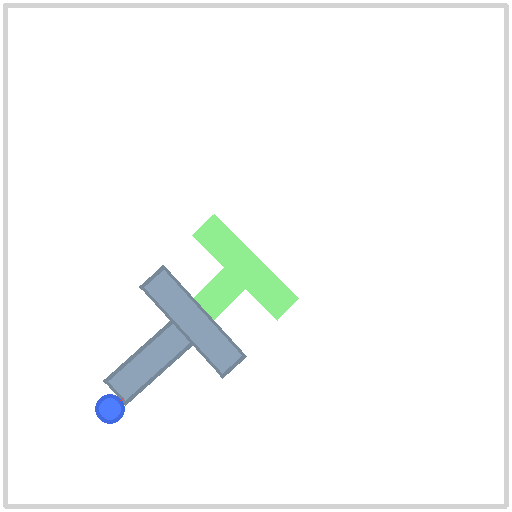
\includegraphics[width=2.05cm]{fig/pusht/prev.png}};
\draw[frame] (prev.south west) rectangle (prev.north east);
\node[img] (cur) at (0.18,3.44) {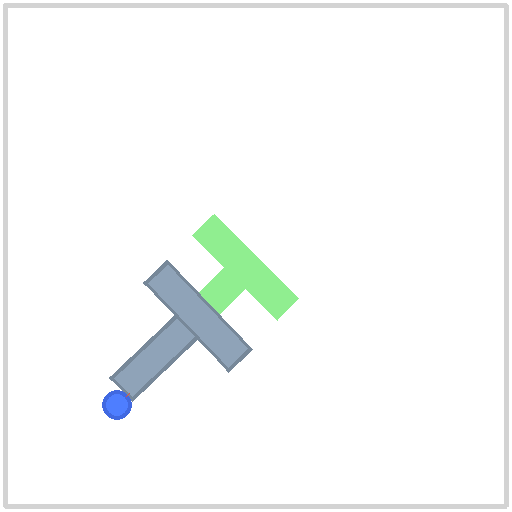
\includegraphics[width=2.05cm]{fig/pusht/cur.png}};
\draw[frame] (cur.south west) rectangle (cur.north east);
\begin{scope}[shift={(0.18,3.44)}, x=2.05cm, y=2.05cm]\draw[zoombox] \FigZoomProp;\end{scope}
\node[lab] at (1.25,3.24) {observations $o_{t-1}, o_t$};
% frozen encoder and policy
\node[frozen] (enc) at (3.3,6.0) {DINOv2 $f$\\[-1pt]{\scriptsize frozen}};
\node[frozen] (pi) at (3.3,4.5) {policy $\pi$\\[-1pt]{\scriptsize frozen}};
\draw[flow] (1.05,5.67) |- (enc.west);
\draw[flow] (2.23,4.5) -- (pi.west);
\node (C) at (4.6,6.0) {$C$};
\draw[flow] (enc) -- (C);
% proposals (zoomed crop)
\node[img] (props) at (4.25,3.44) {\FigImgProp{2.2cm}{cur.png}};
\begin{scope}[shift={(4.25,3.44)}, x=2.2cm, y=2.2cm]\FigPathsProp\end{scope}
\draw[zoombox] (props.south west) rectangle (props.north east);
\node[lab] at (5.35,3.24) {$K{=}8$ proposals $\bA^{(k)}$};
\draw[flow] (pi.east) -- (props.west |- pi.east);
% world model
\node[ours, minimum width=2.05cm] (wm) at (7.75,4.54) {world model\\$p_\theta(S\mid C,\bA)$\\[-1pt]{\scriptsize one batched pass}};
\draw[flow] (6.45,4.54) -- (wm.west);
\draw[flow] (C.east) -- (7.75,6.0) -- (wm.north);
\fill (7.75,6.0) circle (0.9pt);
% 16-token means, one row per proposal
\begin{scope}[shift={(9.22,5.035)}]
  \FigPredCodes
  \foreach \k in {1,...,8} {\node[font=\tiny, anchor=east, inner sep=1pt] at (-0.02,{-(\k-1)*\FigRH+0.5*\FigCellH}) {\k};}
  \draw[black, line width=0.5pt] (-0.02,{-(\FigChosen-1)*\FigRH-0.02}) rectangle ({15*\FigCW+\FigCellW+0.02},{-(\FigChosen-1)*\FigRH+\FigCellH+0.02});
\end{scope}
\draw[flow] (wm.east) -- (9.02,4.54);
\node[lab] at (10.05,3.62) {16-token means $\hat S^{(k)}$};
% reader and goal images
\node[learned, minimum width=1.7cm] (reader) at (11.9,4.54) {reader\\$D_\psi(C,\hat S,g)$\\[-1pt]{\scriptsize inputs: $C,\hat S,g$}};
\draw[flow] (10.93,4.54) -- (reader.west);
\draw[flow] (7.75,6.0) -- (11.35,6.0) -- (11.35,0 |- reader.north);
\foreach \g [count=\i from 0] in \FigGoals {
  \node[img] (goal\i) at ({12.3+0.1*\i},{5.45-0.1*\i}) {\includegraphics[width=0.78cm]{fig/pusht/goal\g.png}};
  \draw[frame] (goal\i.south west) rectangle (goal\i.north east);
}
\node[lab, anchor=west] at (13.45,5.85) {goal images\\$g\in\cG$};
\draw[flow] (12.62,5.25) -- (12.62,0 |- reader.north);
% scores
\begin{scope}[shift={(12.98,5.035)}]
  \FigBars
  \draw[black, line width=0.5pt] (-0.02,{-(\FigChosen-1)*\FigRH-0.02}) rectangle ({\FigBW+0.02},{-(\FigChosen-1)*\FigRH+\FigCellH+0.02});
\end{scope}
\draw[flow] (reader.east) -- (12.94,4.54);
\node[lab] at (13.55,3.62) {scores $s_k$};
% execute
\node[img] (after) at (15.05,3.44) {\FigImgTop{2.1cm}{c\FigChosenIdx s8.png}};
\begin{scope}[shift={(15.05,3.44)}, x=2.1cm, y=2.1cm]\FigChosenTop\end{scope}
\draw[frame] (after.south west) rectangle (after.north east);
\draw[flow] (14.2,4.54) -- node[lab, above] {argmax} (after.west |- 0,4.54);
\node[lab] at (16.1,3.24) {after executing $\bA^{(\FigChosen)}$};
\draw[flow] (after.east |- 0,4.54) -- (17.32,4.54) -- (17.32,2.92) -- node[lab, fill=white, inner sep=1pt, pos=0.3] {observe and replan every $L$ steps} (0.03,2.92) -- (0.03,3.62);

% ============================ training
\begin{scope}[on background layer]
  \fill[black!3, rounded corners=3pt] (-0.06,-0.4) rectangle (17.38,2.68);
  \draw[black!25, rounded corners=3pt] (-0.06,-0.4) rectangle (17.38,2.68);
\end{scope}
\node[anchor=north west, font=\footnotesize\bfseries] at (-0.02,2.64) {(b) Learning the future target (training only)};
% actual futures of two sibling proposals, frames after steps 2, 4, 6, 8
\foreach \s [count=\j from 0] in {2,4,6,8} {
  \node[img] (fa\j) at ({0.75+1.03*\j},1.25) {\FigImgBottom{0.98cm}{c\FigBestIdx s\s.png}};
  \draw[frame] (fa\j.south west) rectangle (fa\j.north east);
  \node[img] (fb\j) at ({0.75+1.03*\j},0.12) {\FigImgBottom{0.98cm}{c\FigWorstIdx s\s.png}};
  \draw[frame] (fb\j.south west) rectangle (fb\j.north east);
}
\node[align=center, inner sep=0pt] at (0.36,1.74) {$\tau^{(\FigBest)}$\\[1pt]{\tiny\FigErrBest\,px}};
\node[align=center, inner sep=0pt] at (0.36,0.61) {$\tau^{(\FigWorst)}$\\[1pt]{\tiny\FigErrWorst\,px}};
\node[lab] at (2.8,-0.17) {frames after steps 2, 4, 6, 8};
% target encoder
\node[learned, minimum width=1.6cm, minimum height=1.9cm] (tenc) at (5.85,1.175) {target\\encoder\\$q_\phi(C,\tau)$};
\draw[flow] (4.83,1.74) -- (tenc.west |- 0,1.74);
\draw[flow] (4.83,0.61) -- (tenc.west |- 0,0.61);
\draw[flow] (5.85,2.6) -- (tenc.north);
\node[font=\scriptsize, anchor=west, inner sep=1pt] at (5.9,2.47) {$C$};
% codes of the actual futures, aligned with the world model above
\begin{scope}[shift={(6.91,1.684)}]\FigSourceCodeA\end{scope}
\begin{scope}[shift={(6.91,0.554)}]\FigSourceCodeB\end{scope}
\draw[flow] (tenc.east |- 0,1.74) -- (6.88,1.74);
\draw[flow] (tenc.east |- 0,0.61) -- (6.88,0.61);
\node[lab] at (7.74,1.08) {FSQ codes $S$};
\draw[aux] (wm.south |- 0,1.83) -- (wm.south);
\node[lab, anchor=west, inner sep=1pt] at (7.82,2.36) {stop-gradient target};
% heads
\node[learned, align=left, minimum height=1.9cm, text width=3.55cm] (heads) at (10.74,1.175) {reader $D_\psi$\\[-1pt]{\scriptsize ranks siblings by progress $\ell$}\\[4pt]feature decoder $G_\xi$\\[-1pt]{\scriptsize reconstructs $f(\tau)$ from $(C,S)$}};
\draw[flow] (8.62,1.74) -- (heads.west |- 0,1.74);
\draw[flow] (8.62,0.61) -- (heads.west |- 0,0.61);
% losses
\node[anchor=west, align=left] at (12.85,1.175) {$\mathcal{L}_{\mathrm{source}}$ (rank + features + saturation)\\[-1pt]{\scriptsize stage 1: target encoder, reader, decoder}\\[4pt]
$\mathcal{L}_{\mathrm{WM}}=\mathcal{L}_{\mathrm{NLL}}+\mathcal{L}_{\mathrm{cons}}+\mathcal{L}^{\hat S}_{\mathrm{rank}}$\\[-1pt]{\scriptsize stage 2: world model}\\[4pt]
{\scriptsize target: 16 tokens, FSQ levels $(8,8,4)$}};
\end{tikzpicture}
